\documentclass[11pt,border=2mm]{standalone}
\usepackage{csquotes}
\usepackage[backend=biber,style=numeric,sorting=none]{biblatex}

\providecommand{\FigScale}{0.75}

\usepackage{siunitx}
\usepackage{tikz}
\usetikzlibrary{decorations.pathmorphing,patterns}
\usetikzlibrary{shapes.geometric, arrows}
\usetikzlibrary{positioning}
 
\usepackage{amsmath}
 
\usepackage{tikz-3dplot}
\usetikzlibrary{3d}
 
\usepackage[siunitx,american]{circuitikz}
 
\usepackage{pgfplots}
\usepgfplotslibrary{units}
\usepgfplotslibrary{groupplots}
\pgfplotsset{compat=1.14}
 
\ctikzset{tripoles/mos style/arrows}
\begin{document}

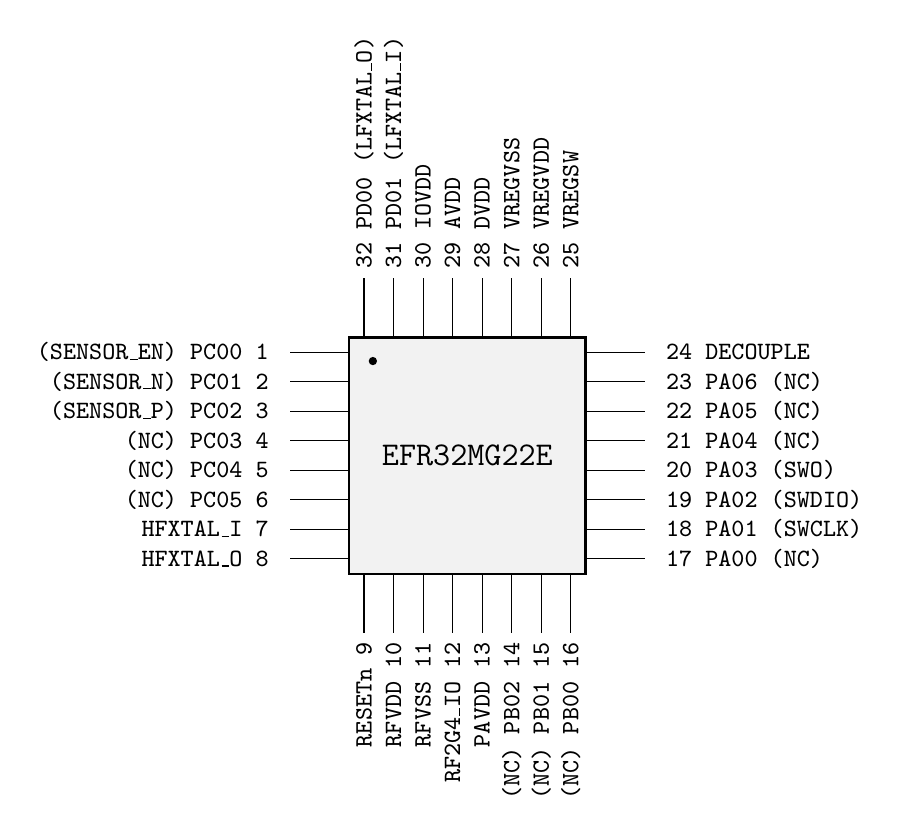
\begin{tikzpicture}[scale=\FigScale, font=\small]

% MCU body
\draw[thick, fill=gray!10] (-2,-2) rectangle (2,2);
\node at (0,0) {\large\texttt{EFR32MG22E}};

% Left side pins (1-8)
\foreach \y/\p in {
  1.75/{\texttt{(SENSOR\_EN) PC00 1}},
  1.25/{\texttt{(SENSOR\_N) PC01 2}},
  0.75/{\texttt{(SENSOR\_P) PC02 3}},
  0.25/{\texttt{(NC) PC03 4}},
  -0.25/{\texttt{(NC) PC04 5}},
  -0.75/{\texttt{(NC) PC05 6}},
  -1.25/{\texttt{HFXTAL\_I 7}},
  -1.75/{\texttt{HFXTAL\_O 8}}
}
{
  \draw (-2,\y) -- (-3,\y);
  \node[left] at (-3.2,\y) {\p};
}

% Bottom side pins (9-16)
\foreach \x/\p in {
  -1.75/{\texttt{RESETn 9}},
  -1.25/{\texttt{RFVDD 10}},
  -0.75/{\texttt{RFVSS 11}},
  -0.25/{\texttt{RF2G4\_IO 12}},
   0.25/{\texttt{PAVDD 13}},
   0.75/{\texttt{(NC) PB02 14}},
   1.25/{\texttt{(NC) PB01 15}},
   1.75/{\texttt{(NC) PB00 16}}
}
{
  \draw (\x,-2) -- (\x,-3);
  \node[below, rotate=90, anchor=east] at (\x,-3) {\p};
}

% Right side pins (17-24)
\foreach \y/\p in {
  -1.75/{\texttt{17 PA00 (NC)}},
  -1.25/{\texttt{18 PA01 (SWCLK)}},
  -0.75/{\texttt{19 PA02 (SWDIO)}},
  -0.25/{\texttt{20 PA03 (SWO)}},
   0.25/{\texttt{21 PA04 (NC)}},
   0.75/{\texttt{22 PA05 (NC)}},
   1.25/{\texttt{23 PA06 (NC)}},
   1.75/{\texttt{24 DECOUPLE}}
}
{
  \draw (2,\y) -- (3,\y);
  \node[right] at (3.2,\y) {\p};
}

% Top side pins (25-32)
\foreach \x/\p in {
   1.75/{\texttt{25 VREGSW}},
   1.25/{\texttt{26 VREGVDD}},
   0.75/{\texttt{27 VREGVSS}},
   0.25/{\texttt{28 DVDD}},
  -0.25/{\texttt{29 AVDD}},
  -0.75/{\texttt{30 IOVDD}},
  -1.25/{\texttt{31 PD01 (LFXTAL\_I)}},
  -1.75/{\texttt{32 PD00 (LFXTAL\_O)}}
}
{
  \draw (\x,2) -- (\x,3);
  \node[above, rotate=--90, anchor=west] at (\x,3) {\p};
}

% Pin 1 marker
\fill (-1.6,1.6) circle (2pt);

\end{tikzpicture}

\end{document}